%%
%% This is file `sample-sigconf.tex',
%% generated with the docstrip utility.
%%
%% The original source files were:
%%
%% samples.dtx  (with options: `sigconf')
%% 
%% IMPORTANT NOTICE:
%% 
%% For the copyright see the source file.
%% 
%% Any modified versions of this file must be renamed
%% with new filenames distinct from sample-sigconf.tex.
%% 
%% For distribution of the original source see the terms
%% for copying and modification in the file samples.dtx.
%% 
%% This generated file may be distributed as long as the
%% original source files, as listed above, are part of the
%% same distribution. (The sources need not necessarily be
%% in the same archive or directory.)
%%
%% The first command in your LaTeX source must be the \documentclass command.
\documentclass[sigconf]{acmart}
\usepackage[spanish]{babel}
\usepackage[utf8]{inputenc}
\usepackage{lmodern}
\usepackage{tabularx}
\usepackage{listings}




%%
%% \BibTeX command to typeset BibTeX logo in the docs
\AtBeginDocument{%
	\providecommand\BibTeX{{%
			\normalfont B\kern-0.5em{\scshape i\kern-0.25em b}\kern-0.8em\TeX}}}





%%
%% end of the preamble, start of the body of the document source.
\begin{document}
	
	%%
	%% The "title" command has an optional parameter,
	%% allowing the author to define a "short title" to be used in page headers.
	\title{Práctica 1}
	
	%%
	%% The "author" command and its associated commands are used to define
	%% the authors and their affiliations.
	%% Of note is the shared affiliation of the first two authors, and the
	%% "authornote" and "authornotemark" commands
	%% used to denote shared contribution to the research.
	\author{Jorge Humberto Sierra Florido}
	\email{2123065656@cua.uam.mx}
	\affiliation{
		\institution{UAM Cuajimalpa \\ Ingeniería en Computación}
		\city{Ciudad de México}
		\country{México}
	}
	
	\author{María de Jesús Sánchez Zepeda}
	\email{2153068423@cua.uam.mx}
	\affiliation{
		\institution{UAM Cuajimalpa\\ Ingeniería en Computación}
		\city{Ciudad de México}
		\country{México}
	}
	
	%%
	%% The abstract is a short summary of the work to be presented in the
	%% article.
	\begin{abstract}
		%  Aqu{\'i} va el abstract de la pr{\'a}ctica...
	\end{abstract}
	
	%%
	%% This command processes the author and affiliation and title
	%% information and builds the first part of the formatted document.
	\maketitle
	
	\section{Introducción}
	
	Al tener un \textit{dataset} en ocasiones no se cuentan con todos los campos llenos por lo que antes de realizar el análisis de los datos es importante la limpieza de ellos. El término limpieza se refiere al tratamiento que se dara al \textit{dataset} para sustituir los datos faltantes con el fin de no inducir un sesgo en el modelo generado mediante el ánalisis de los datos.
	
	Para encontrar relaciones entre dos variables continuas definidas en la misma población se puede utilizar el coeficiente de correlación y la regresión lineal. En está práctica se tienen dos conjuntos de datos de diferentes tamaños a los cuáles se les desea encontrar un modelo una ecuación que modele la relación entre variables determinadas. Para ello se limpiaron los datos de cada conjunto, posteriormente se generaron los diagramas de dispersión que ayudan a identificar los \textit{outliers}. Después se realizó una regresión lineal para generar un modelo, el cual posteriormente se evaluó mediante el cálculo de la eficiencia del modelo generado y el grado de error que contiene.
	
	%Texto introductorio al tema en que se enfoca la pr{\'a}ctica y lo que se desarrollar{\'a} en ella. Se debe escribir un texto que introduzca el tema de la 
	%pr{\'a}ctica, definici{\'o}n del problema, los objetivos, motivaci{\'o}n,  y resultados esperados.
	
	\section{Conceptos previos}
	
	%Escribir conceptos te{\'o}ricos empleados en el desarrollo de la pr{\'a}ctica (f{\'o}rmulas matem{\'a}ticas, por ejemplo). Es un tipo de secci{\'o}n con todos los conceptos te{\'o}ricos empleados.
	Dependiendo del tipo de variables $\mathbb{x_{1},...x_{n}}$ los modelos lineales se pueden clasificar en: 
	\begin{itemize}
		\item{Análisis de la Varianza del modelo} cuando la matriz \textbf{X} tiene únicamente ceros y unos, es decir, son cualitativas.
		\item{Modelo de Regresión} si todas las variables son cuantitativas.
		\item{Análisis de la Covarianza del modelo} cuando algunas variables son son (0,1), es decir, cualitativas y otras son cuantitativas.
	\end{itemize}
	\subsection{Modelo de regresión lineal}
	El Modelo de regresión lineal nos permite saber la correlación entre dos variables asumiendo que la varianza es constante en la población. Dados $\overrightarrow{\beta}, \overrightarrow{x} \epsilon$$\mathbb{R}^{m+1}$, el modelo de regresión lineal se establece según la ecuación (1).
	\begin{equation}
		\hat{y}=h_{\overrightarrow{B}}(\overrightarrow{x})=\beta_{0}x_{0}+\beta_{1}x_{1}\mathrm{+...+}\beta_{m} x_{m}=\overrightarrow{\beta}^T \cdot \overrightarrow{x}  
	\end{equation}
	donde, $m$: número de características, $x_{i}$ i-ésima característica, $\beta_{i}$ i-ésimo parámetro del modelo, $\hat{y}$: valor predicho, $h_{\overrightarrow{\beta}}$ función de hipótesis, usando parámetros del modelo $\overrightarrow{\beta}$
	\subsubsection{Regresión lineal no ponderada
	}
	En caso de que en la población a estudiar la varianza no sea uniforme la regresión lineal mediante mínimos cuadrados ponderados da predicciones poco fiables. En este caso, si las diferencias de variabilidad se pueden pronosticar a partir de otra variable se puede utilizar el procedimiento de Estimación ponderada que contrasta un rango de transformaciones de ponderación e indica cuál da mejores predicciones
	\subsection{Error cuadrático Medio}
	La función de error cuadrático medio \textit{MSE} se usa como criterio de evaluación en problemas de regresión debido a que cada dato obtenido mediante la regresión lineal se puede comparar con el valor real. Se puede calcular mediante la fórmula (2).
	\begin{equation}
		MSE\left(\mathbf{X},h_{\overrightarrow{\beta}}\right)  =
		\frac{1}{n}   \mathbf{\Sigma} \sum_{i=1}^n \left(h_{\overrightarrow{\beta}}\left(\overrightarrow{x_{i}}\right)-y_{i}\right)^2
	\end{equation}
	donde $\hat{y}$$=h_{\overrightarrow{\beta}}\left(\overrightarrow{x_{i}}\right)=\overrightarrow{\beta}^T \cdot \overrightarrow{x_{i}}$
	\section{Metodología}
	
	Se analizaron los \textit{datasets} usando el lenguaje de programación R\footnote{R es un lenguaje orientado a computo estadístico y de gráficas, \url{https://www.r-project.org/} } y el IDE R studio. a fin de generar los resúmenes estadísticos y gráficas requeridas, esto tras limpiarlos de información faltante.
	
	Posteriormente se procedió al análisis de la información usando \textit{Python}, ayudándonos de \textit{Scikit-Learn, Pandas} y \textit{Numpy}.
	Se requirió investigar la función \textit{LinearRegression}, para aplicarla a los \textit{datasets} y generar los modelos
	
	Finalmente se evaluaron los modelos y se compararon la regresión lineal normal y la ponderada.
	
	\section{Resultados}
	
	Se inicio la practica revisando los \textit{datasets} proporcionados, estos corresponden a los datos de temperatura y salinidad medidas, así como las características de algunos vehículos. 
	
	El primer paso fue cargar los datos en R a fin de poder analizar los datasets. para esta carga se usaron las instrucciones del Código \ref{lst:cargaDatos}
	
	\begin{lstlisting}[caption=lectura de los datos,breaklines,label=lst:cargaDatos]
		data = read.csv("water.csv", header=TRUE)
		data2 = read.table("mtcars.txt", header=TRUE )
	\end{lstlisting}
	
	Una vez cargada la información se procedió a obtener el resumen de la misma con la siguiente instrucción del Código \ref{lst:resumen1}, generando la salida mostrada en la Tabla \ref{tab:Tabla1}
	
	\begin{lstlisting}[caption=Resumen de los datos,breaklines,label=lst:resumen1]
		summary(data)
	\end{lstlisting}
	
	\begin{table}
		\begin{tabularx}{\columnwidth}{|X|X|X|X|}
			\hline
			\multicolumn{2}{|c|}{ TdegC } & \multicolumn{2}{|c|}{ Salnty }  \\
			\hline
			Min. & 1.44  & Min. & 28.43 \\
			\hline
			1st Qu.& 7.68 &1st Qu.&33.49 \\
			\hline
			Median &10.06  & Median & 33.86   \\
			\hline
			Mean & 10.80 & Mean & 33.84\\
			\hline
			3rd Qu.&13.88 & 3rd Qu. & 34.20\\
			\hline
			Max. & 31.14 & Max.& 37.03  \\
			\hline
			NA's & 10963 & NA's  & 47354\\
			\hline
		\end{tabularx}
		\caption{\label{tab:Tabla1}Resumen de el dataset water.csv}
	\end{table}
	
	En la Tabla \ref{tab:Tabla1} se observaron 10963 registros vacíos en el campo de temperatura y 47354 en la salinidad.
	Se eligió como alternativa dejar los elementos con campos NA, remplazándolos por su Mediana, esto para no afectar el \textit{dataset}. Este remplazo se realizo usando el Código \ref{lst:remplazo1}
	
	\begin{lstlisting}[caption=Código de emplazo de los NA,breaklines,label=lst:remplazo1]
		data$Salnty[is.na(data$Salnty)] = 33.86
		data$TdegC[is.na(data$TdegC)] = 10.06
	\end{lstlisting}
	
	El nuevo resumen genero la Tabla \ref{tab:Tabla2} Donde se observan cambios mínimos.
	
	\begin{table}
		\begin{tabularx}{\columnwidth}{|X|X|X|X|}
			\hline
			\multicolumn{2}{|c|}{ TdegC } & \multicolumn{2}{c|}{ Salnty }  \\
			\hline
			Min. & 1.44  & Min. & 28.43 \\
			\hline
			1st Qu.& 7.72 &1st Qu.&33.50 \\
			\hline
			Median &10.06  & Median & 33.86   \\
			\hline
			Mean & 10.79 & Mean & 33.84\\
			\hline
			3rd Qu.&13.83 & 3rd Qu. & 34.18\\
			\hline
			Max. & 31.14 & Max.& 37.03  \\
			\hline
		\end{tabularx}
		\caption{\label{tab:Tabla2}Resumen limpio de el dataset water.csv}
	\end{table}
	
	Respecto a los datos de el \textit{dataset} de carros posterior a su carga, se requirió filtrar solo los campos relevantes usando el Código \ref{lst:seleccion} y se obtuvo posteriormente el Resumen en la Tabla \ref{tab:Tabla3}. Con el resumen observamos que este dataset no tiene datos faltantes, procederemos a trabajar con el así.
	
	\begin{lstlisting}[caption=Código de seleccion de las propiedades,breaklines,label=lst:seleccion]
		data2 = subset(data2, select=c(4,5,7))
	\end{lstlisting}
	
	\begin{table}
		\begin{tabularx}{\columnwidth}{|X|X|X|X|}
			\hline
			& hp & disp & wt \\
			\hline
			Min.   & 52.0  & 71.1 & 1.513   \\
			\hline
			1st Qu.& 96.5 & 120.8 & 2.581   \\
			\hline
			Median & 123.0 & 196.3 & 3.325    \\
			\hline
			Mean   & 146.7 & 230.7 & 3.217   \\
			\hline
			3rd Qu. & 180.0 & 326.0 & 3.610  \\
			\hline
			Max.  & 335.0 & 472.0 & 5.424  \\
			\hline
		\end{tabularx}
		\caption{\label{tab:Tabla3}Resumen de el dataset mtcars.txt}
	\end{table}
	
	En los BoxPlot de las propiedades Temperatura (Figura \ref{fig:temperaturaBP}) y la Salinidad (Figura \ref{fig:salinidadBP}) se observan sus outliers en Rojo
	
	\begin{figure}
		\centering
		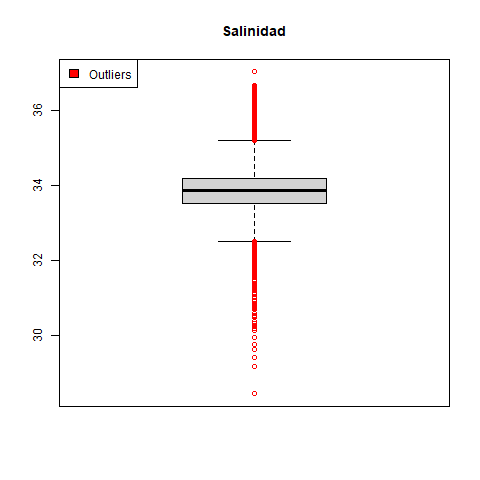
\includegraphics[width=0.7\linewidth]{img/salinidad.png}
		\caption{Boxplot de la propiedad Salinidad en water}
		\label{fig:salinidadBP}
	\end{figure}
	
	\begin{figure}
		\centering
		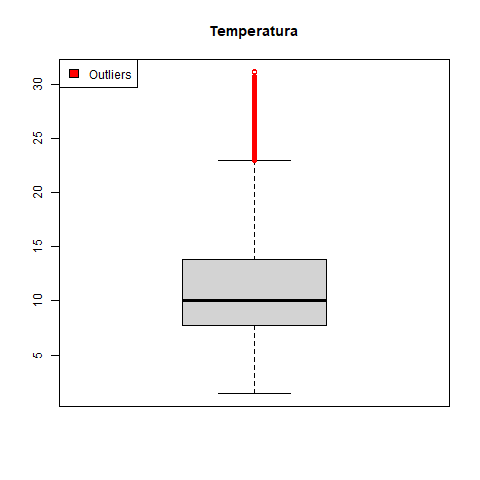
\includegraphics[width=0.7\linewidth]{img/temperatura.png}
		\caption{Boxplot de la propiedad Temperatura en water}
		\label{fig:temperaturaBP}
	\end{figure}
	
	
	En las Figuras (\ref{fig:hpBP},\ref{fig:wtBP} y\ref{fig:dispBP}) podemos ver las Boxplot de las propiedades HP (Horse Power), wt (weigth) y disp (Displacement) respectivamente
	
	\begin{figure}
		\centering
		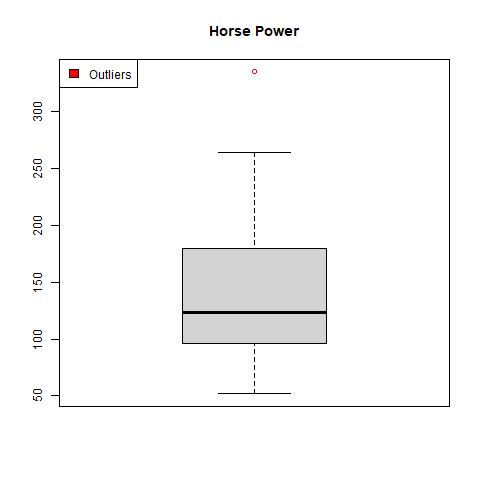
\includegraphics[width=0.7\linewidth]{img/hpBoxplot.png}
		\caption{Boxplot de la propiedad hp en mtcars}
		\label{fig:hpBP}
	\end{figure}
	
	\begin{figure}
		\centering
		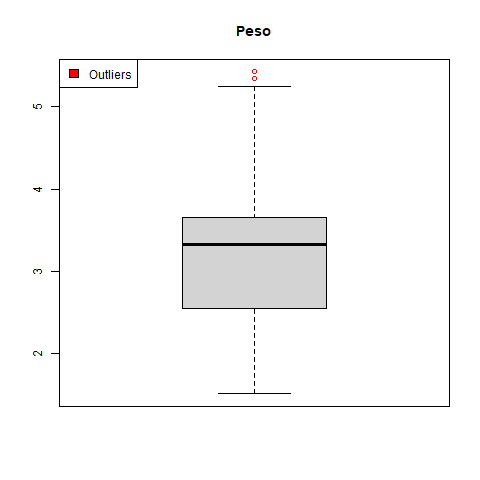
\includegraphics[width=0.7\linewidth]{img/wtBoxplot.png}
		\caption{Boxplot de la propiedad wt en mtcars}
		\label{fig:wtBP}
	\end{figure}
	
	\begin{figure}
		\centering
		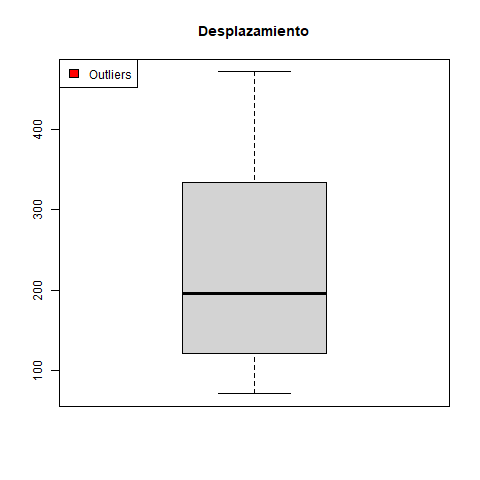
\includegraphics[width=0.7\linewidth]{img/dispBoxplot.png}
		\caption{Boxplot de la propiedad disp en mtcars}
		\label{fig:dispBP}
	\end{figure}
	
	Para observar mas caracteristicas de la informacion del dataset water, se obtuvo la grafica de dispersion entre el valor de entrada (Salinidad) y el valor de salida (Temperatura), esto se observa en la Figura \ref{fig:waterD}
	
	\begin{figure}
		\centering
		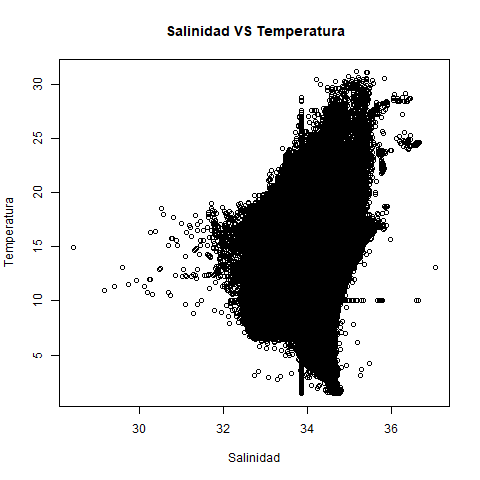
\includegraphics[width=0.7\linewidth]{img/dispersionSalinidadVSTemperatura.png}
		\caption{Dispersión de los datos de Salinidad Vs Temperatura}
		\label{fig:waterD}
	\end{figure}
	
	El caso de la gráfica de dispersión nos proporciono un ejemplo interesante de lo que ocurre al pedirle graficar datasets con mas de una característica. La primera aproximación fue mandar el dataset completo a graficar la Figura \ref{fig:carsD1} donde se observo que la función de graficado genera una gráfica compuesta de subgraficas colocando cada característica contra las demás, omitiendo las de la propiedad consigo misma.
	
	\begin{figure}
		\centering
		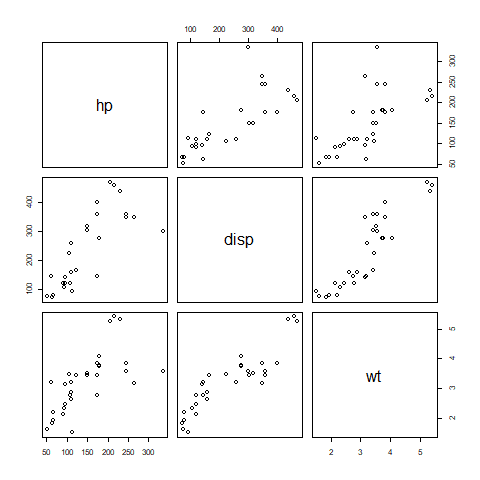
\includegraphics[width=0.7\linewidth]{img/dispersionCarros.png}
		\caption{Primera grafica de dispersion generada}
		\label{fig:carsD1}
	\end{figure}
	
	A fin de apreciar mejor las graficas y tomando en cuenta que los datos de entrada son el disp y wt para predecir hp, así que se genero las graficas de cada dato de entrada contra el dato de salida resultando las Figuras (\ref{fig:carsD2A}, \ref{fig:carsD2B})
	
	\begin{figure}
		\centering
		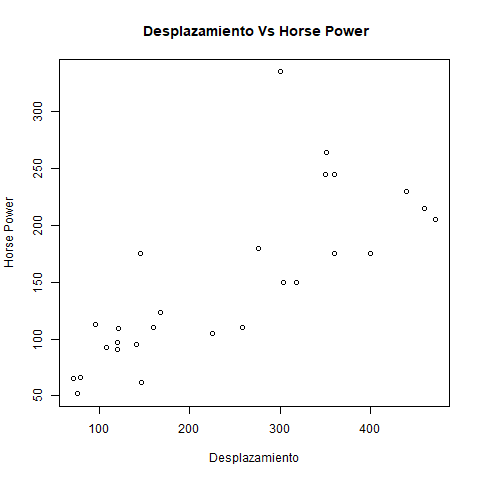
\includegraphics[width=0.7\linewidth]{img/dispersionCarrosHPVSDISP.png}
		\caption{Gráfica de dispersión HP vs DISP}
		\label{fig:carsD2A}
	\end{figure}
	
	\begin{figure}
		\centering
		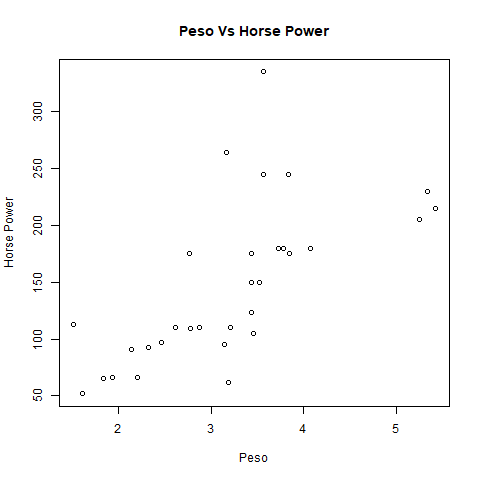
\includegraphics[width=0.7\linewidth]{img/dispersionCarrosHPVSWT.png}
		\caption{ Gráfica de dispersión HP vs WT}
		\label{fig:carsD2B}
	\end{figure}
	
	Despues se procedio a investigar la documentacion de la funcion LinearRegression de Scikit-learn, dicha funcion recibe 5 parametros
	
	\begin{itemize}
		\item \verb|fit_intercept| Se usa para definir si se usara un interceptor en los calculos
		\item \verb|normalize| Normalizara los datos antes de entrar a la programacion del modelo
		\item \verb|copy_X|  Define si la operacion sera destructiva o no sobre el set de datos original
		\item \verb|n_jobs| Se usa para indicar cuantos trabajos se usaran para esta computacion, Se usa cuando la cantidad de objetivos es mayor a 1
		\item \verb|positive| Forza a que los coeficientes a ser positivos
	\end{itemize}
	
	Para el dataset mayor se uso la metodología simple, usando una proporción de 80-20 de proporción para el training set y el test set.
	
	Para la generación de estos sets, se uso otra función de Scikit-learn, la función \verb|train_test_split| \ref{lst:set8020}, de esta función nos interesan los siguientes parámetros
	
	\begin{itemize}
		\item \verb|test_size| Un valor en el rango (0,1) que indica el tamaño porcentual del set de pruebas
		\item \verb|train_size| Un valor en el rango (0,1) que indica el tamaño porcentual del set de entrenamiento
		\item \verb|random_state| Un valor que puede ser un entero o un generador de numeros aleatorios, para garantizar la repetibilidad se puede usar el mismo valor numerico
	\end{itemize}
	
	\begin{lstlisting}[caption=Código de emplazo de los NA,breaklines,label=lst:set8020]
		x_train, x_test, y_train, y_test = train_test_split(x, y, test_size=0.2, train_size=0.8, random_state=42)
	\end{lstlisting}
	
	Una vez realizada esta división se procede a generar el modelo entrenandolo con el training set usando el metodo fit , posterior a esto se usara el set de pruebas y se comparo lo generado por el modelo y lo establecido en el set de pruebas. En la Figura \ref{fig:waterSimpleVal} graficamos los datos de el set de prueba en color negro y los de color azul los valores del modelo.
	
	\begin{figure}
		\centering
		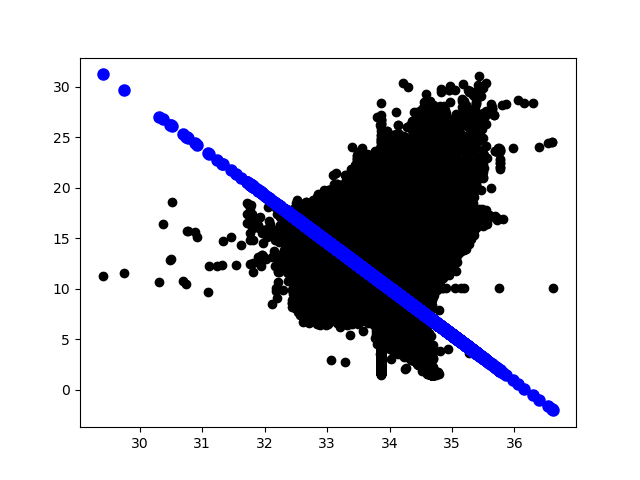
\includegraphics[width=0.7\linewidth]{img/validacionSimpleWater.png}
		\caption{Gráfica comparando la predicion contra el set de prueba}
		\label{fig:waterSimpleVal}
	\end{figure}
	
	Para el dataset de cars se uso el mecanismo de N fold, el cual nos solicita generar N conjuntos de prueba y entrenamiento. Para generarlos se uso la funcion
	
	
	\section{Conclusiones y reflexiones}
	
	%Conclusiones generales de la pr{\'a}ctica. A\~nadir una reflexi{\'o}n anal{\'i}tica por cada miembro del equipo.
	\subsection{Conclusión}
	\subsection{Reflexiones}
	\subsubsection{Jorge Sierra}
	\subsubsection{María Sánchez}
	%%
	%% The next two lines define the bibliography style to be used, and
	%% the bibliography file.
	\bibliographystyle{ACM-Reference-Format}
	\bibliography{references}
	
	
\end{document}
\endinput
%%
%% End of file `sample-sigconf.tex'.
